\documentclass{article}
\usepackage[top=0.5in, bottom=0.5in, left=1.25in, right=1.25in]{geometry}

\usepackage{amsmath, array, enumerate, sfmath, pgfplots, pgfplotstable, tcolorbox, graphicx, color, colortbl, multicol}
\pgfplotsset{compat = newest}
\usepgfplotslibrary{statistics}
\usetikzlibrary{arrows.meta}
\renewcommand{\familydefault}{\sfdefault}
\raggedright
\pagestyle{empty}

\newcounter{example}[section]
\newenvironment{example}[1][]{\refstepcounter{example}\par\medskip
   {\color{red}\textbf{Example~\theexample. #1}}}{\medskip}

\begin{document}

\section*{Probability: AND}

\begin{tcolorbox}[colframe=orange!70!white, coltitle=black, title=\textbf{Summary}]
\begin{enumerate}
    \item Typically, the word \texttt{and} indicates multiplication.
    \item In general, $P(A \text{ and } B = P(A) \times P(B | A)$.
\end{enumerate}
\end{tcolorbox}
\vspace{0.75in}

\begin{example}
You flip a coin and then roll a single die. What is the probability that you flip heads {\color{blue}\textbf{and}} roll a 5?
\end{example}
\vspace{1in}

\subsection*{Multiplication Rule}

In the previous example, the probability of flipping heads was $\frac{1}{2}$	\newline\\	
The probability of rolling a 5 was $\frac{1}{6}$	
\vspace{1in}
\begin{tcolorbox}[colframe=green!20!black, colback = green!30!white,title=\textbf{Multiplication Rule}]
If $P(A)$ is the probability of event $A$ occurring, and $P(B)$ is the probability of event $B$ occurring, then
\[P(A\text{ and } B) = P(A) \times P(B)\]
\end{tcolorbox}

\vfill 

\subsection*{Tree Diagrams}

\begin{center}
\tikzstyle{level 1} = [level distance = 3cm, sibling distance = 10cm]
\tikzstyle{level 2} = [level distance = 3cm, sibling distance = 1.25cm]
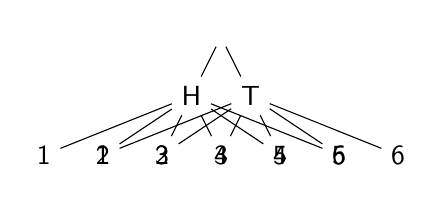
\begin{tikzpicture}[scale=0.5]
\node {}
	child {node {H}
		child {node {1}}
		child {node {2}}
		child {node {3}}
		child {node {4}}
		child {node {5}}
		child {node {6}}}
	child {node {T}{
		child {node {1}}
		child {node {2}}
		child {node {3}}
		child {node {4}}
		child {node {5}}
		child {node {6}} }
		};
\end{tikzpicture}
\end{center}

\vfill 
\newpage 

\subsection*{Venn Diagrams: AND}
\vspace{0.25in}

\begin{center}
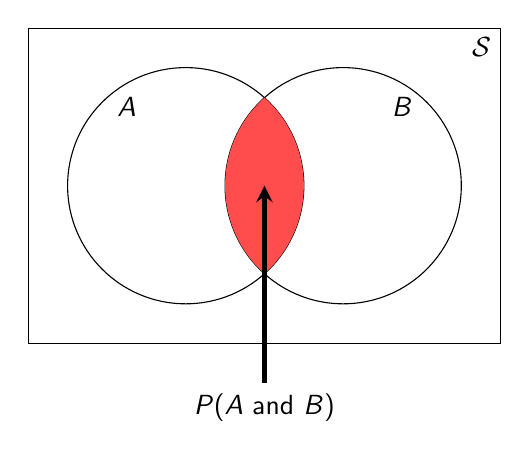
\begin{tikzpicture}
\def\circleA{(2,2) circle [radius = 1.5cm]} 
\def\circleB{(4,2) circle [radius = 1.5cm]} 
\draw (0,0) rectangle (6,4) node [below left] {$\mathcal{S}$};
\draw \circleA;
\node at (1.25,3) {$A$};
\draw \circleB;
\node at (4.75,3) {$B$};
\begin{scope}
\clip \circleA;
\fill[red!70] \circleB;
\end{scope}
\draw [<-, >=stealth, ultra thick] (3,2) -- (3,-0.5) node [below] {$P(A\text{ and } B)$};
\end{tikzpicture}
\end{center}

\vfill 

\begin{center}
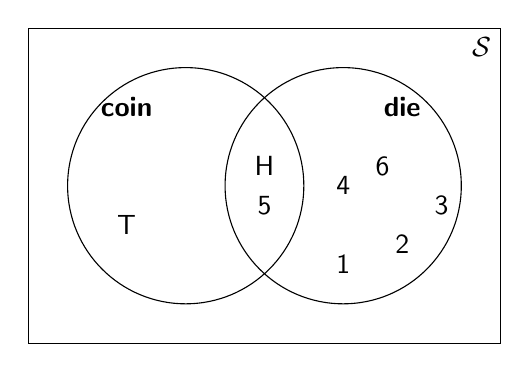
\begin{tikzpicture}
\def\circleA{(2,2) circle [radius = 1.5cm]} 
\def\circleB{(4,2) circle [radius = 1.5cm]} 
\draw (0,0) rectangle (6,4) node [below left] {$\mathcal{S}$};
\draw \circleA;
\node at (1.25,3) {\textbf{coin}};
\draw \circleB;
\node at (4.75,3) {\textbf{die}};
\node at (1.25,1.5) {T};
\node at (3,2.25) {H};
\node at (3,1.75) {5};
\node at (4,1) {1};
\node at (4.75,1.25) {2};
\node at (5.25,1.75) {3};
\node at (4,2) {4};
\node at (4.5,2.25) {6};
\end{tikzpicture}
\end{center}

\vfill 

\begin{tcolorbox}[colframe=green!20!black, colback = green!30!white,title=\textbf{Mutually Exclusive Events}]
Two events are \textbf{mutually exclusive} if they can not happen together. In other words,
\[P(A\text{ and } B) = 0\]
\end{tcolorbox}

\vfill 
\newpage 

\subsection*{Independent Events}
\vspace{0.25in}

\begin{tcolorbox}[colframe=green!20!black, colback = green!30!white,title=\textbf{Independent Events}]
Two events are \textbf{independent} if the outcome of the second is not affected by the first happening.
\end{tcolorbox}
\vspace{0.5in}

\[P(A \text{ and } B) = P(A) \times P(B)\]

\vspace{0.5in}

When selecting items from a collection, independent events often contain selections made {\color{blue}\textbf{\underline{with replacement}}}.

\vspace{1in}

\begin{example}
A jar contains 10 blue, 12 black, and 15 red marbles.
\begin{enumerate}[(a)]
    \item What is the probability of selecting a black marble, putting it back, and then selecting a blue marble?    \vfill 
    \item What is the probability of selecting a red marble, putting it back, and then selecting another red marble?   \vfill
\end{enumerate}
\end{example}

\begin{example}
A certain blood test can determine the presence of a bloodborne pathogen 97\% of the time (that is, if 100 people have the pathogen, the test will confirm true for 97 of them). If 4 people with the pathogen are given the test, find the probability that the test is accurate for all of them.
\end{example}

\vfill 
\newpage 

\subsection*{Conditional Probability}

\vspace{0.25in}

\begin{tcolorbox}[colframe=green!20!black, colback = green!30!white,title=\textbf{Conditional Probability}]
\textbf{Conditional probability} limits a sample space and is found by determining a probability \emph{based on a previous event happening}.
\end{tcolorbox}

\vspace{0.5in}

The notation for the probability that event $B$ occurs given that event $A$ has occurred is
\[ P(B \mid A)\]

\vspace{1in}

With conditional probability, the denominator will often be the total of something that follows the words ``if", ``suppose", or ``given that".
\vspace{1in}

\begin{example}
The table below lists the types and numbers of cars sold at Lemon Autos along with their ages. Find each probability.	\newline\\
\begin{center}
\begin{tabular}{c|ccccc}
					&	\textbf{0--2} & \textbf{3--5} & \textbf{6--10} & \textbf{Over 10} & \textbf{Total} \\ \hline
\textbf{Import} 	& 37 & 21 & 12 & 30 & 100 \\
\textbf{Domestic} 	& 35 & 23 & 11 & 31 & 100 \\ \hline
\textbf{Total}   	& 72 & 44 & 23 & 61 & 200
\end{tabular}
\end{center}

\begin{enumerate}[(a)]
    \item If a domestic car is randomly selected, what is the probability that it is 6--10 years old?    \vfill 
    \item What is the probability of selecting a domestic car given that the car is 6--10 years old?  \vfill 
    \item Suppose a new car is selected, what is the probability that it is an import?
\end{enumerate}
\end{example}

\vfill 
\newpage 

\subsection*{Dependent Events}

\vspace{0.25in}

\begin{tcolorbox}[colframe=green!20!black, colback = green!30!white,title=\textbf{Dependent Events}]
Two events are \textbf{dependent} if the outcome of the second is affected by the first happening.
\end{tcolorbox}
\vspace{1in}

Dependent events utilize conditional probability:
\[P(A\text{ and } B) = P(A) \times P(B \mid A)\]

\vspace{0.5in}

\emph{Note}: When selecting items from a collection, dependent events often contain selections made {\color{blue}\textbf{\underline{without replacement}}}.

\vspace{1in}

\begin{example}
You are dealt a card from a standard deck and then you are dealt another (without replacement). Find each probability.
\begin{enumerate}[(a)]
    \item The first card is an ace and the second card is a ten.   \vfill 
    \item The first card is an ace and the second card is an ace.  \vfill 
\end{enumerate}
\end{example}

\newpage 

\subsection*{Conditional Probability Revisited}
\vspace{0.25in}

The formula for dependent events
\[P(A\text{ and } B) = P(A) \times P(B \mid A)\]
leads us to the following formula for conditional probability:
\[P(B \mid A) = \frac{P(A \text{ and } B)}{P(A)}\]

\vspace{0.5in}

When finding \texttt{AND} probabilities using tabular data
\begin{itemize}
    \item Look for the intersection of a row and column.
    \item Two rows (likewise, two columns) will never intersect, so their probabilities are \emph{mutually exclusive}.
\end{itemize}

\vspace{0.75in}

\begin{example}
The table below lists the types and numbers of cars sold at Lemon Autos along with their ages. Find each probability.	\newline\\
\begin{center}
\begin{tabular}{c|ccccc}
					&	\textbf{0--2} & \textbf{3--5} & \textbf{6--10} & \textbf{Over 10} & \textbf{Total} \\ \hline
\textbf{Import} 	& 37 & 21 & 12 & 30 & 100 \\
\textbf{Domestic} 	& 35 & 23 & 11 & 31 & 100 \\ \hline
\textbf{Total}   	& 72 & 44 & 23 & 61 & 200
\end{tabular}
\end{center}

\begin{enumerate}[(a)]
    \item If a car is randomly selected, what is the probability that it is a 6--10 year old import?     \vfill 
    \item If a car is randomly selected, what is the probability that it is a domestic car that is 0--2 years old?     \vfill
    \item If a car is randomly selected, what is the probability that it is 0--2 years and 6--10 years old?    \vfill 
\end{enumerate}
\end{example}



\end{document}
